\scanpage{23}
\figure{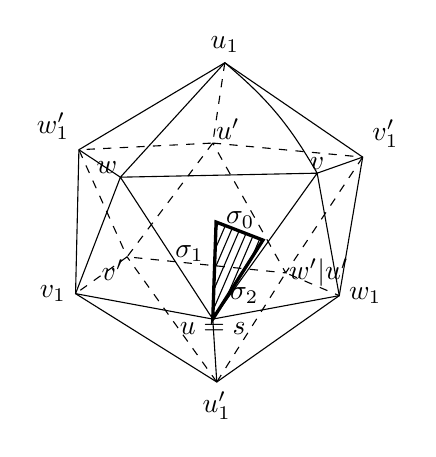
\begin{tikzpicture}[x=.85cm,y=.85cm]
\coordinate (ut) at (0,3); \coordinate (lt) at (-2.18,1.70); \coordinate (rt) at (2.06,1.59);
\coordinate (lb) at (-2.23,-.45); \coordinate (rb) at (1.71,-.48); \coordinate (bt) at (-.12,-1.77);
\coordinate (w) at (-1.56,1.29); \coordinate (v) at (1.38,1.35); \coordinate (u) at (-.18,-.83);
\coordinate (up) at (-.18,1.8); \coordinate (vp) at (-1.46,.10); \coordinate (wp) at (.91,-.14);
\draw (ut)--(lt)--(lb)--(bt)--(rb)--(rt)--cycle;
\draw[dashed] (up)--(vp)--(wp)--cycle (ut)--(up)--(lt)--(vp)--(lb)
 (bt)--(vp) (bt)--(wp)--(rb) (rt)--(wp) (up)--(rt);
\draw (w)--(v)--(u)--cycle (ut)--(w)--(lt) (lb)--(w) (lb)--(u)--(bt)
 (u)--(rb)--(v)--(rt) (ut) to[bend left=10] (v);
\coordinate (b) at (-.13,.62); \coordinate (c) at (.57,.35);
\begin{scope}\clip (u)--(b)--(c)--cycle;
\foreach \x in {-1.0,-.88,...,1.0}{\draw[thin] (\x,-.94)--++(.80,1.86);}
\end{scope}
\draw[very thick] (u)--(b)--(c)--cycle;
\node[above] at (ut) {$u_1$}; \node[above left] at (lt) {$w'_1$};
\node[above right] at (rt) {$v'_1$}; \node[left] at (lb) {$v_1$};
\node[right] at (rb) {$w_1$}; \node[below] at (bt) {$u'_1$};
\node[above left,inner sep=1pt] at (w) {$w$}; \node[above,inner sep=1pt] at (v) {$v$};
\node[below,inner sep=1pt] at (u) {$u=s$}; \node[above right,inner sep=1pt] at (up) {$u'$};
\node[below left,inner sep=1pt] at (vp) {$v'$}; \node[right,inner sep=1pt] at (wp) {$\unsure{w'|u'}$};
\node[above,inner sep=1pt] at (.23,.48) {$\sigma_0$}; \node[left] at (-.17,.15) {$\sigma_1$};
\node[right,inner sep=1pt] at (.03,-.48) {$\sigma_2$};
\end{tikzpicture}}

$\sigma_1$ et $\sigma_2$ fixent $s$, donc \deleted{conservent l'orientation de} \inserted{induisent des permutations} paires de $T$. D'autre part $\sigma_0$ conserve le troisième sommet $w$ (opposé à $a$) de la face (triangulaire) $f$, donc par ce qui précède \deleted{conserve} \inserted{induit} \unsure{égalt|ég\textsuperscript{t}} une orientation paire de $T$. Donc

\uline{Corollaire} $G=\mathrm{Aut}(\Pi)$ opère sur $T$ par permutations paires, i.e. on a
\[
G\longrightarrow\mathrm{Alt}_{T\deleted{\unsure{E}}}
\]
Comme $u\in G$, $s\in S$ implique évidemment
\[
\omega_{u(s)}=u(\omega_s)
\]
il s'ensuit, $G$ étant transitif sur $S$

\uline{Corollaire} Les orientations $\omega_s$ $(s\in S)$ de $T$ associées aux $s\in S$ sont ttes égales.

D'où une \uline{orientation} \uline{canonique sur} $T$ (évidemment conservée par $G=\mathrm{Aut}(\Pi)$).
% archive sheet number: 22
